\chapter{Strawman Mission \& Instrument Configuration}
% See awesome notes by "Johannes Linde"
\autsection{Strawman proposal}{Paschalis Dalampiras}
\begin{figure}[htb!]
\centering
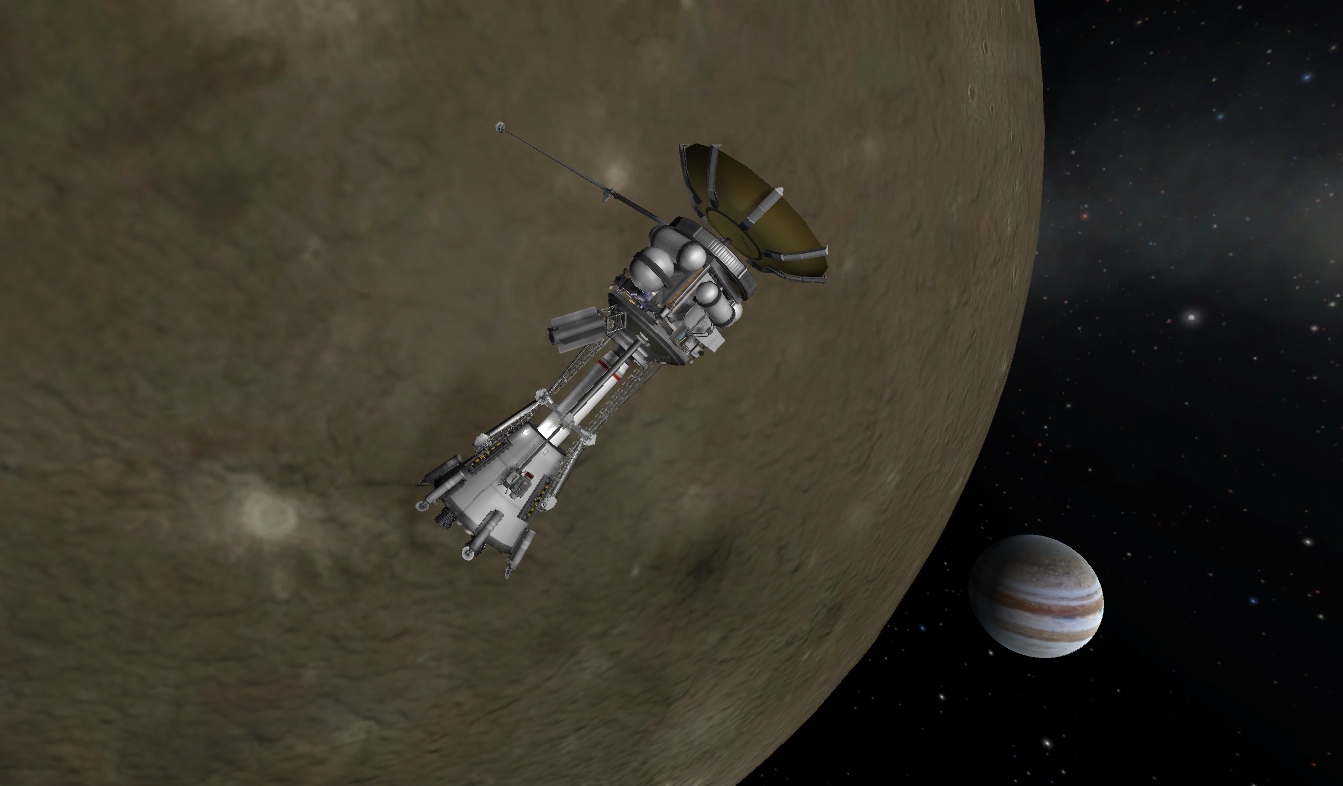
\includegraphics[width=\textwidth]{figures/Orbiter/9.PNG}
\caption{Spacecraft concept design, before orbiter-lander separation, performing a targeted encounter of Ganymede. (Kerbal Space Program)}
\label{fig:spacecraft}
\end{figure}

\newpage 
\subsection{Orbiter Concept}

\begin{figure}[htb!]
\centering
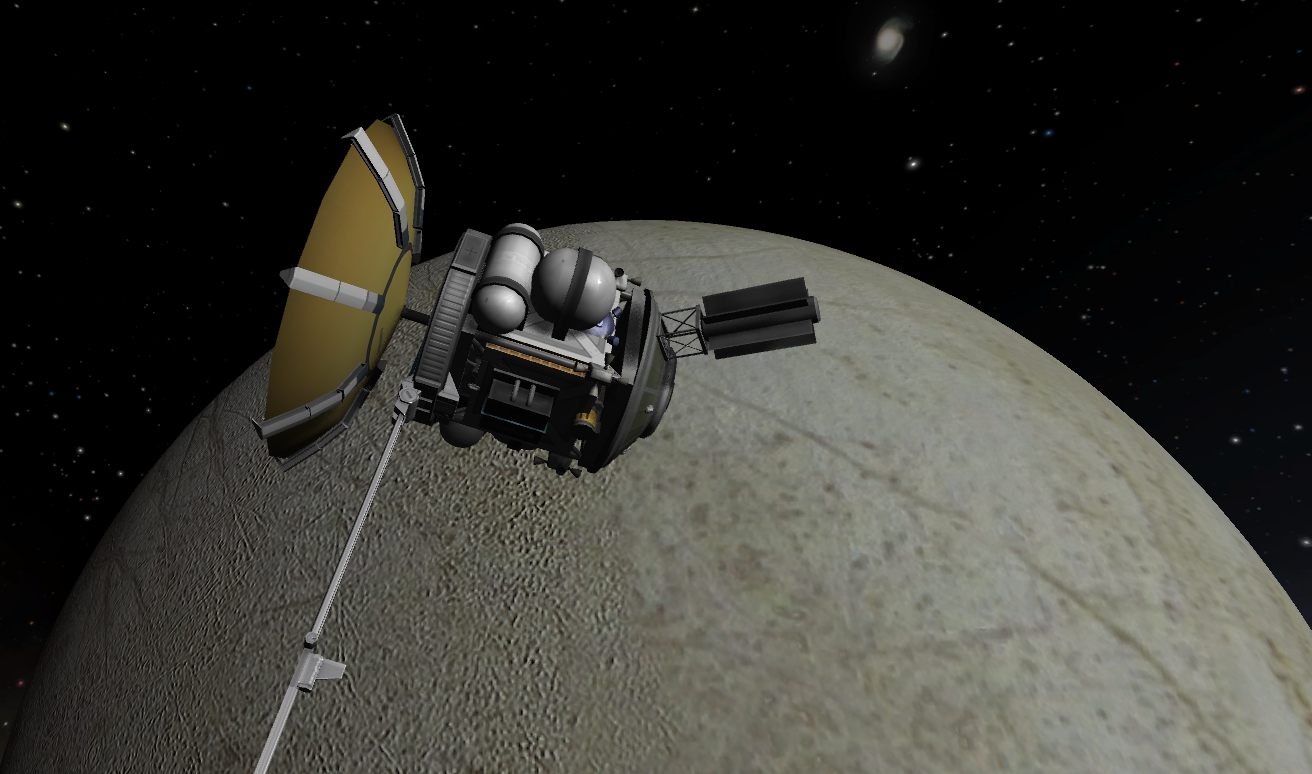
\includegraphics[width=\textwidth]{figures/Orbiter/orbiter.PNG}
\caption{Orbiter concept design, performing a flyby of Europa.(Kerbal Space Program)}
\label{fig:orbiter}
\end{figure}

\subsubsection{Orbiter Science}
Orbiter was designed to conduct a number of measurements to provide an insight into some of the geophysical characteristics that make Europa a unique environment of great scientific interest. Local topography of the moon’s volatile icy surface coupled with thickness measurements of the ice crust will expand the geological knowledge. Additionally, magnetic field measurements will reveal information of the induced magnetic field of Europa. As a secondary task, orbiter has also been assigned on collecting geophysical data of Ganymede and Calisto, taking advantage of the necessary flybys along these moons.

\subsubsection{Orbiter Mission Concept}
Conducting the planned measurements will require a set of remote sensing instruments (Optical spectroscopy camera, ground penetrating radar) as well as in situ instruments (Magnetometer) mounted on radiation shielded spacecraft capable of enduring the high radiation environment. Measurements will be carried out from varying altitudes ranging from 500km to 100km depending on the orbit sequence, providing local high resolution mapping of surface locations with high interest and investigating Europa’s magnetic field. 

\subsubsection{Orbiter Mission Design}
The spacecraft will be launched on a Delta IV Heavy rocket placing it into an interplanetary trajectory. A Gravity Assist Venus-Mars-Venus-Earth will guide the orbiter into a Jupiter Orbit Insertion after 3.7 years (Anastassios E. Petropoulos et al. 2000) where over the span of 165 days six gravity assist flybys of Ganymede and Europa will reduce the orbital delta v and place it into a highly elongated orbit around Jupiter. Performing a technique will set the orbiter in resonance orbit in respect to Europa. Orbit selection was based on the principal of avoiding long exposure over the area where radiation belts are more intense while on the same time allowing the craft to perform close flybys in resonance to Europa in order to complete the science observations.

\subsection{Lander Concept}

\begin{figure}[htb!]
    \centering
    \captionsetup[subfigure]{width=0.45\textwidth}
    \subfloat{
        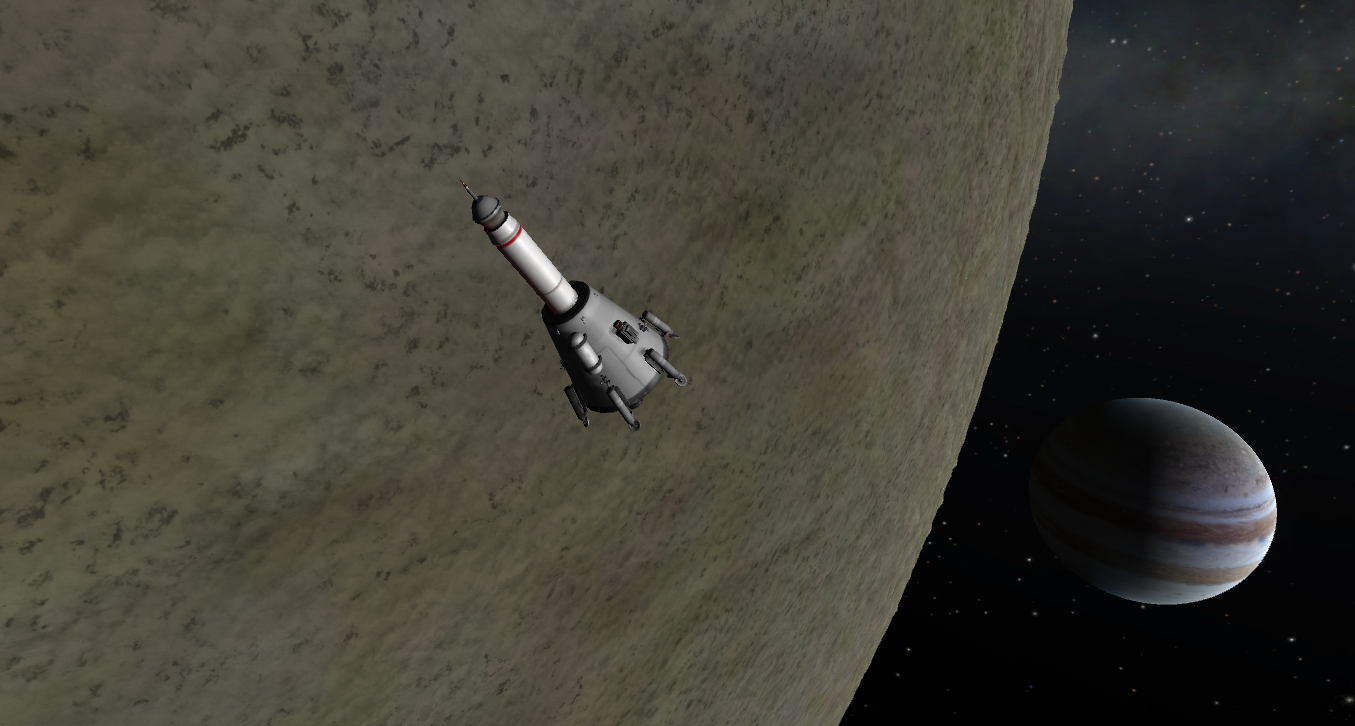
\includegraphics[width=.48\textwidth]{figures/Orbiter/2.PNG}
    }
    \subfloat{
        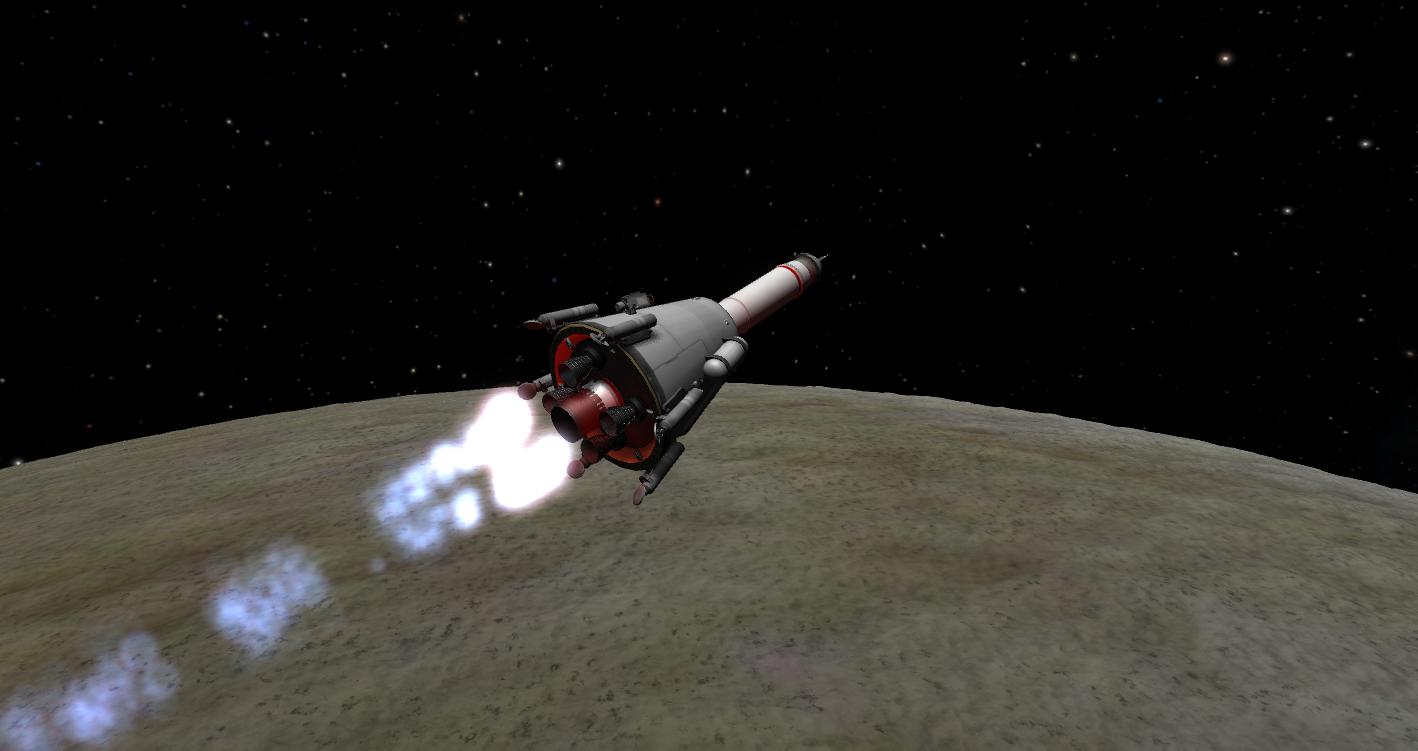
\includegraphics[width=.48\textwidth]{figures/Orbiter/4.PNG}
    }
    \caption{Lander concept design, preparing for descent.(Kerbal Space Program)}
\end{figure}

\subsubsection{Lander Science}

Main objective of the lander is to act as a secure and sufficient carrier of the designed penetrator, which will conduct a series of in situ experiments beneath the ice surface. Onboard surface cameras will provide high resolution images of the surface area and of the landing site, while microphones will record low amplitude sounds from potentially geological activity.

\subsubsection{Lander Mission Concept}
A highly radiation tolerant lander, capable of withstanding the blasting radiation in the near Jupiter environment will be deployed on the surface of Europa, delivering the penetrator safely and fulfilling the main goal of the mission. 
After acquiring data of topography and ice thickness measurements from the orbiter, a safe landing site will be manually selected after a reconnaissance campaign. A set of reconnaissance cameras will aid the landing while an angering system will secure the lander after landing, an essential system considering the low gravity environment of Europa. In order to facilitate the penetrator’s descent through the ice, main engines will be used to sublimate the top surface layer of the ice. Communication between orbiter-lander and lander-penetrator will be established using a set of two antennas with sufficient bandwidth for reliable telemetry.

\subsubsection{Lander Mission Design}

Lander will be launched attached to the carrier spacecraft, following the main trajectory sequence of the latter as described on the orbiter mission design.  
Release from the orbiter will be initiated at an altitude of 100km which will commence the descent phase. A micro-ASC unit is responsible for landing guidance, tracking the relative position of the lander. Two laser based devices, one for estimating the altitude range and one which will act as a structured light hazard avoidance system will assist the landing phase. An anchoring system will be deployed on touchdown, securing the lander from departing while a short burn of the main engines will use remaining fuel upon depletion to rapture the top layer of surface ice and prepare the conditions for the penetrator deployment. 

\subsection{Ice Penetrator Concept}

\begin{figure}[htb!]
\centering
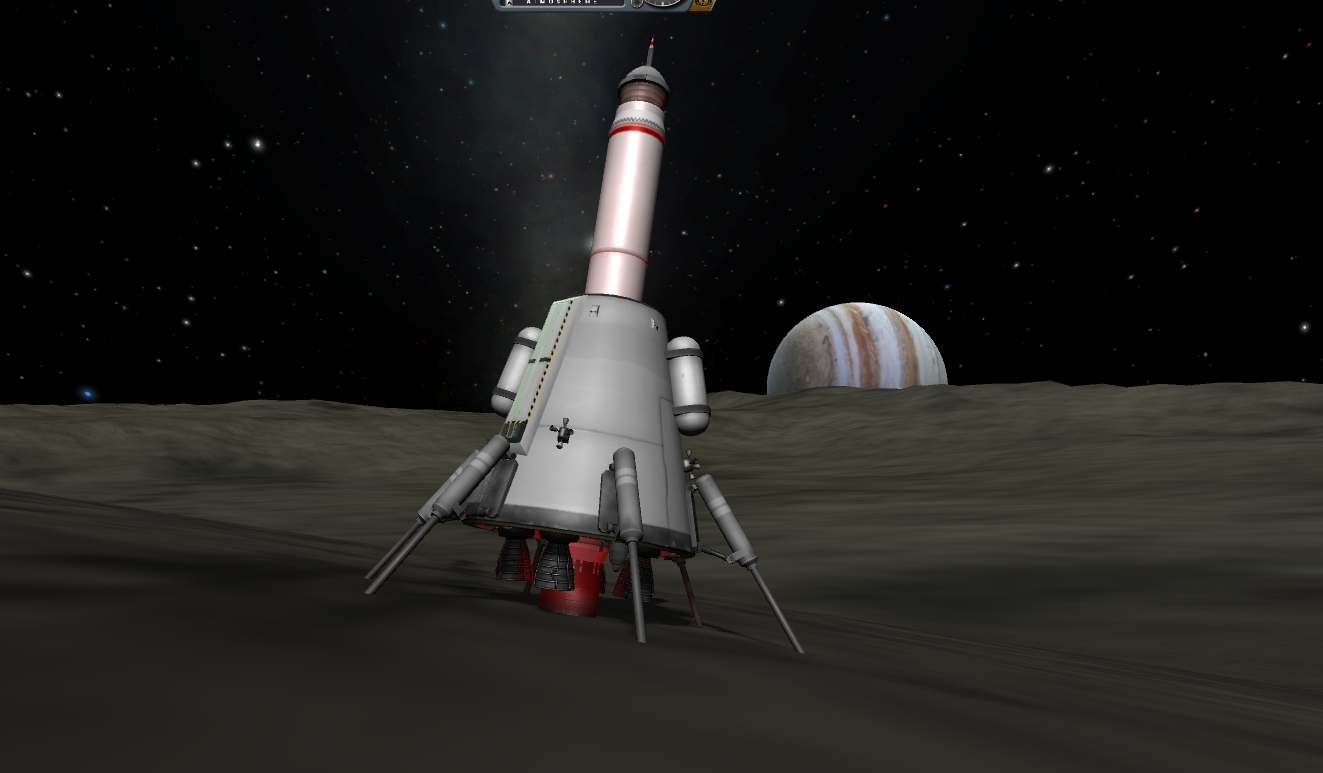
\includegraphics[width=\textwidth]{figures/Orbiter/8.PNG}
\caption{Lander with the penetrator deployed, preparing for the drilling phase. (Kerbal Space Program)}
\label{fig:penetrator}
\end{figure}

\subsubsection{Ice Penetrator Science}

Europa life finder mission concept relies on in-situ observations of the potential liquid water ocean beneath the icy surface of the moon. The highest priority objective of the mission is focused on detecting and analyzing potential life presence with the use of highly sophisticated and efficient scientific instruments. Secondary objectives include, investigation of the water composition by analyzing acquired samples as well as investigation of the ocean’s chemistry and characteristics of the water.
Science objectives are listed below.


\subsubsection{Ice Penetrator Mission Concept}

Measurements are carried out through a single location between the lower limit of the ice shell and the surface of the ocean. In-situ observations are conducted on the top layer of the ocean using a set of instruments deployed directly into the water.
Planned payload consists of nine instruments, a Mass Spectrometer, an Acoustic Doppler current profiler (ADCP), a Water Filtering System, a Microscopic Imager, a Barometer, a Thermometer, a Camera and a Microphone.

\subsubsection{Ice Penetrator Mission Design}

All the essential measurements will be conducted via a -torpedo shaped- self-propelled by gravity vehicle, capable of transferring and deploying the instruments beneath the floating icy shell that surrounds Europa. The ice crust is estimated to be several kilometers thick, thereat thermal power provided by an on-board Radioisotope Thermoelectric Generator (RTG) will be used to rupture and melt a 20-cm wide borehole through the ice, as the unit descents on higher depths. While descending, small size transceivers will be deployed and attached to the inner wall of the borehole in order to relay communications from the penetrator to the lander. Once penetrator has reached the surface of the under-ice ocean, an anchoring system will secure the vehicle on the ice and instruments will be deployed for the planned measurements. Acquired data will be relayed back to the orbiter through the transceivers and the lander’s communication system. 
